% Conception générale du système

\section{Organisation générale du système}

\subsection{Organisation au niveau du site}

\subsubsection{Fonctionnalités principales}
Les cuves seront équipées de capteurs qui communiqueront avec un système
embarqué en temps réel. Ce capteur sera adapté en fonction des besoins, il
existe de nombreux capteurs sur le marché d'après l'étude de l'existant. Le
système embarqué pourra : 

\begin{itemize}
\item \textbf{connaître sa position} Avec le signal GPS reçu avec son module GPS
\item \textbf{s'alimenter en énergie} au travers de batterie, éolienne ou
de panneaux solaires selon les contraintes environnementales définies par
le milieu pour être en autonomie et communiquer l'énergie crée au système
embarqué
\item \textbf{connaître l'information} fournie par le capteur
\item \textbf{communiquer} avec le serveur central ainsi que localement
avec les propriétaires ou les compagnies d'entretien. Cette communication
avec le serveur central sera faite par le biais des réseaux GSM ou
satellite en cas d'indisponibilité du réseau.
\end{itemize}

\subsubsection{Interactions Possibles}

Il sera possible d'intéragir localement pour les compagnies et les
propriétaires avec un PDA ou un smartphone. Cette communication aura lieu
avec un antenne bluetooth placée au sein du système embarqué.

%avec l'exploitant

\subsection{Organisation au niveau des serveurs}

Les données issues des sites sont reçues par les serveurs et sont stockés
sur le serveur principal. Elles seront accessibles à l'ensemble des
ayant-droits, notamment le COPEVUE, les sociétés en charges des sites
concernés et les prioritaires des sites respectifs. 

Le serveur central s'occupera des traitements. 

\subsection{Organisation au niveau local}

Le COPEVUE, les propriétaires et les sociétés en charge disposeront
d'interfaces adaptés à leur besoin. Elles ne stockeront pas de données
localement, les traitements seront fait sur le serveur central.  Au niveau
local ils pourront reconfigurer les paramètres des capteurs ou des sites au
besoin.  Le serveur central peut faire remonter au niveau local des alertes
(Ex: "Cuve remplie, Cuve vide, Besoin en prévision d'incendies...)

%intégrer le schéma


%\begin{figure}[!h]
%\begin{center}
%    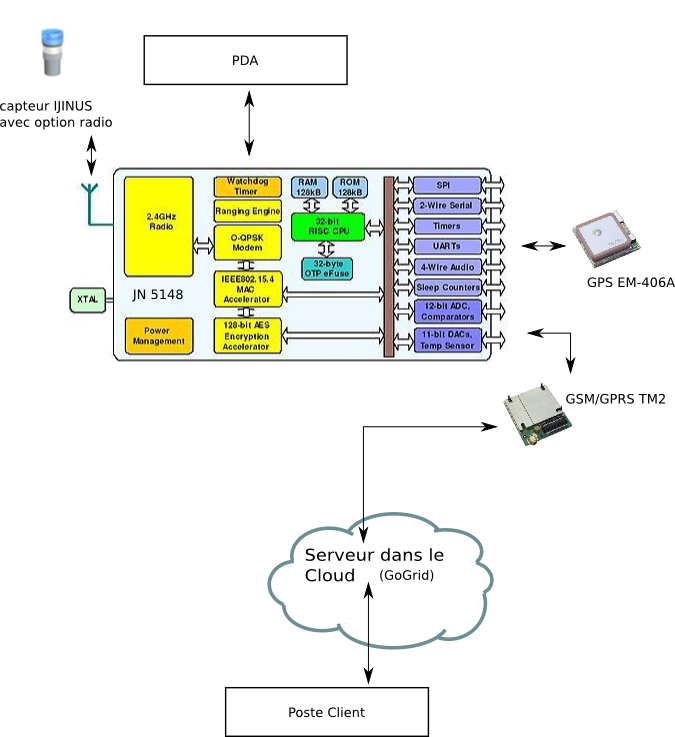
\includegraphics[width=12cm]{\PIXPATH/org-gen}
%\end{center}
%\end{figure}
